% ************ Chapter 3 ************
%\renewcommand{\chaptername}{Chapter}
\chapter{Análise de Valor}
\label{cap:3}
%\emph{Este capítulo incide em apresentar de que forma as diferentes alternativas criam valor para o público alvo, e desta forma tirar conclusões sobre qual alternativa deve ser aprofundada}

A análise das diferentes alternativas de modelos descentralizados apresentados na secção \ref{section_modelos_descentralizados} consolida-se tendo em conta certos parâmetros e tem como objetivo decidir a solução sobre a qual serão dedicados esforços no sentido de criar contribuições com potencial de melhoria de escalabilidade.

\section{Análise de Valor\label{section_analise}}

Aplicando o modelo de Peter A. Koen, \emph{New Concept Development} (\emph{c.f} \ref{subsection_new_concept_development}), é possível mapear uma oportunidade para um conceito, seguindo todos elementos chave do modelo e percebendo assim
se esta oportunidade representa ou não valor para a organização.

\subsection{Identificação da Oportunidade}
Neste contexto, a oportunidade surge no sentido de prevenir o acontecimento de escândalos como o conhecido Cambridge Analytica e outros \emph{“leaks”} \cite{cambridge_analytica} de informação que acontecem a um ritmo cada vez superior numa \emph{Web} baseada num paradigma que parece cada vez mais desajustado para a realidade que vivemos nos dias de hoje.

\subsection{Análise da Oportunidade}
O conceito “descentralização da \emph{Web}” não é novo, mas tem ganho ênfase nos últimos tempos e existem esforços notáveis para tornar este conceito numa realidade e tornar viável o surgimento de uma \emph{Web} mais livre e mais transparente.

Esta dissertação passa inicialmente por perceber que alternativas existem e qual pode ter mais potencial numa vertente de adoção massiva a médio prazo. Os projetos que serão analisados são aqueles que foram abordados com maior destaque no estado da arte (\emph{c.f. secção \ref{section_modelos_descentralizados}}): \emph{Solid}, \emph{Blockstack}, \emph{Diaspora} e \emph{Elastos}.

\subsection{Enriquecimento da ideia}
Nesta fase é importante perceber os fatores que se apresentam como mais relevantes para uma \emph{framework} capaz de potencializar um novo paradigma de \emph{Web} descentralizada:
\begin{itemize}
\item  Gestão de informação - No sentido de prevenir escândalos de acessos indevidos a informação pessoal e combater a monopolização dos dados, existe necessidade de garantir a defesa da sua propriedade.

\item Mecanismo de autenticação e autorização - A propriedade dos dados é assegurada por mecanismos de autenticação e autorização.

\end{itemize}

\subsection{Seleção da ideia}

Para esta componente foi utilizada a técnica \acrshort{AHP} (\emph{c.f.} secção \ref{section_AHP}).

\subsubsection*{Divisão Hierárquica}

A primeira fase desta técnica é apresentar os critérios mais relevantes para a tomada de decisão.

Neste sentido, para perceber qual a relevância de cada critério é apresentada uma tabela com a matriz dos critérios (\emph{c.f.} tabela \ref{table_matriz_criterios}) e a tabela com a matriz de critérios normalizada (\emph{c.f.} tabela \ref{table_matriz_criterios_normalizada}).

\begin{table}[h]
\centering
\caption{Matriz Critérios}
\label{table_matriz_criterios}
\vspace{0.5cm}
\begin{tabular}{c|c|c|c} 
 - & Autenticação & Autorização & Armazenamento \\
\hline                          
Autenticação & 1 & 1 1/2 & 1,75 \\
Autorização &  2/3 & 1 & 1 1/4  \\
Armazenamento &  4/7 & 4/5 & 1 \\
Soma & 2 5/21 & 3 3/10 & 4 \\
\end{tabular}
\end{table}

\begin{table}[h]
\centering
\caption{Matriz Critérios Normalizada}
\label{table_matriz_criterios_normalizada}
\vspace{0.5cm}
\begin{tabular}{c|c|c|c|c} 
 - & Autenticação & Autorização & Armazenamento & Média Ponderada \\
\hline                               
Autenticação & 21/47 & 5/11 & 7/16 & 45\% \\
Autorização &  14/47 & 10/33 & 5/16 & 30\% \\
Armazenamento &  12/47 &  8/33 & 1/4 & 25\% \\
Soma & 1 & 1 & 1 & 100\% \\
\end{tabular}
\end{table}

\pagebreak

\subsubsection*{Definição de Prioridades}
Após os critérios e as devidas prioridades estarem identificadas, segue-se a apresentação das diferentes alternativas, bem como a sua prestação face aos diferentes critérios: Autenticação (tabela 3.3), autorização (tabela 3.4) e armazenamento (tabela 3.5). 

\begin{table}[H]
\centering
\caption{Prioridades Relativas Autenticação}
\vspace{0.5cm}
\begin{tabular}{c|c|c|c|c|c} 
 - & Solid & BlockStack & Diaspora & Elastos & Prioridade Relativa \\
\hline                               
Solid & 41\% &	48\% &	44\% & 33\% \\
BlockStack &  21\% & 24\% &	22\% &	33\% &	25\% \\
Diaspora &  10\% &	12\% &	11\% & 11\%	& 11\% \\
Elastos & 28\% & 16\% & 22\% & 22\% & 22\% \\
\end{tabular}
\end{table}

\begin{table}[H]
\centering
\caption{Prioridades Relativas Autorização}
\vspace{0.5cm}
\begin{tabular}{c|c|c|c|c|c} 
 - & Solid & BlockStack & Diaspora & Elastos & Prioridade Relativa \\
\hline                               
Solid & 26\% &	35\% &	10\% & 45\% & 29\% \\
BlockStack &  18\% & 25\% & 32\% & 21\% & 24\% \\
Diaspora &  43\% &	13\% &	17\% &	10\% & 20\% \\
Elastos & 13\% & 28\% &	42\% & 24\% & 27\% \\
\end{tabular}
\end{table}

\begin{table}[H]
\centering
\caption{Prioridades Relativas Armazenamento}
\vspace{0.5cm}
\begin{tabular}{c|c|c|c|c|c} 
 - & Solid & BlockStack & Diaspora & Elastos & Prioridade Relativa \\
\hline                               
Solid & 23\% & 35\% & 8\% & 44\% & 28\% \\
BlockStack &  17\% & 25\%	& 32\%	& 22\%	& 24\% \\
Diaspora &  47\% &	13\% & 17\%	& 10\% & 22\% \\
Elastos & 13\% & 28\% & 42\% & 24\% & 27\% \\
\end{tabular}
\end{table}

\subsubsection*{Consistência}

\begin{table}[h]
\centering
\caption{Resultados \acrshort{AHP}}
\label{tabela_resultados_ahp}
\vspace{0.5cm}
\begin{tabular}{c|c|c|c|c|c} 
 - & Autenticação & Autorização & Armazenamento & Valor Final & \\
\hline                               
Solid & 42\% &	29\% & 28\%	& 33\% & \\
BlockStack &  25\% & 24\% & 24\% & 24\% & \\
Diaspora &  11\% &	20\% & 22\% & 18\% & \\
Elastos & 22\% & 27\% & 27\% & 25\% & \\
\end{tabular}
\end{table}

Tendo em conta os estudos apresentados na tabela \ref{tabela_resultados_ahp}, o caminho a seguir será aprofundar a framework Solid de forma a torná-la mais escalável e preparada para a uma possível adoção massiva.

\subsection{Definição do Conceito}
O momento da definição do conceito corresponde à fase final da formalização da ideia já escolhida anteriormente. O conceito introduzido pelo Solid, em conjunto com o possível potencial de escalabilidade, permite tornar o conceito de “\emph{Web} Descentralizada” numa realidade.

\section{Proposta de Valor \label{section_proposta_de_valor}}
Para estudar da proposta de valor serão utilizados o modelo \emph{\acrshort{FAST}} (\emph{c.f. secção \ref{subsection_modelo_fast}}) e o modelo de negócio Canvas (\emph{c.f.} secção \ref{subsection_modelo_canvas}).
Estes modelos tem como objetivo ajudar a desenhar o sistema tendo por base objetivos numa perspetiva de negócio e de sustentabilidade.

\subsection{Modelo \emph{\acrshort{FAST}}\label{subsection_modelo_fast}}
Com base na sua representação (\emph{c.f. figura \ref{figura_modelo_fast}} é possível perceber que o “core” de toda framework são os dados e que estes estão sob alçada do seu utilizador, podendo o mesmo a qualquer momento tomar ações como revogar acesso a determinadas aplicações (\emph{relying party} \footnote{\emph{\acrshort{POD}} ou aplicação cliente que utiliza um token providenciado por um servidor de identidade.}).

\begin{figure}[H]
    \begin{center}
    % Requires \usepackage{graphicx}
    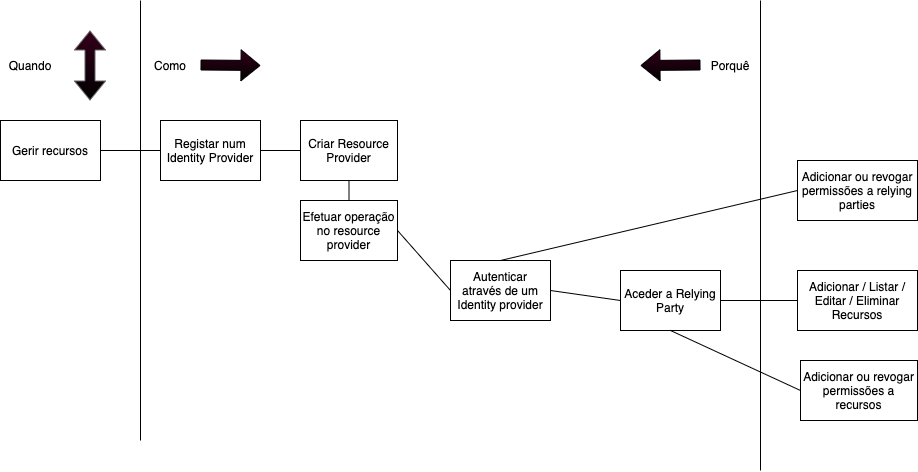
\includegraphics[height=0.4\textwidth]{figures/Canvas-FAST.png}
    \caption{Modelo \emph{\acrshort{FAST}}}
    \label{figura_modelo_fast}
    \end{center}
\end{figure}

\subsection{Modelo Canvas\label{subsection_modelo_canvas}}
O modelo canvas é uma ferramenta de gestão estratégica que permite o desenvolvimento do modelo de negócio para determinado projeto. A sua estrutura conta com nove blocos pré-definidos que permitem, de forma visual, criar ou adaptar um modelo já existente\cite{alexander:2006}.

\begin{figure}[H]
    \begin{center}
    % Requires \usepackage{graphicx}
    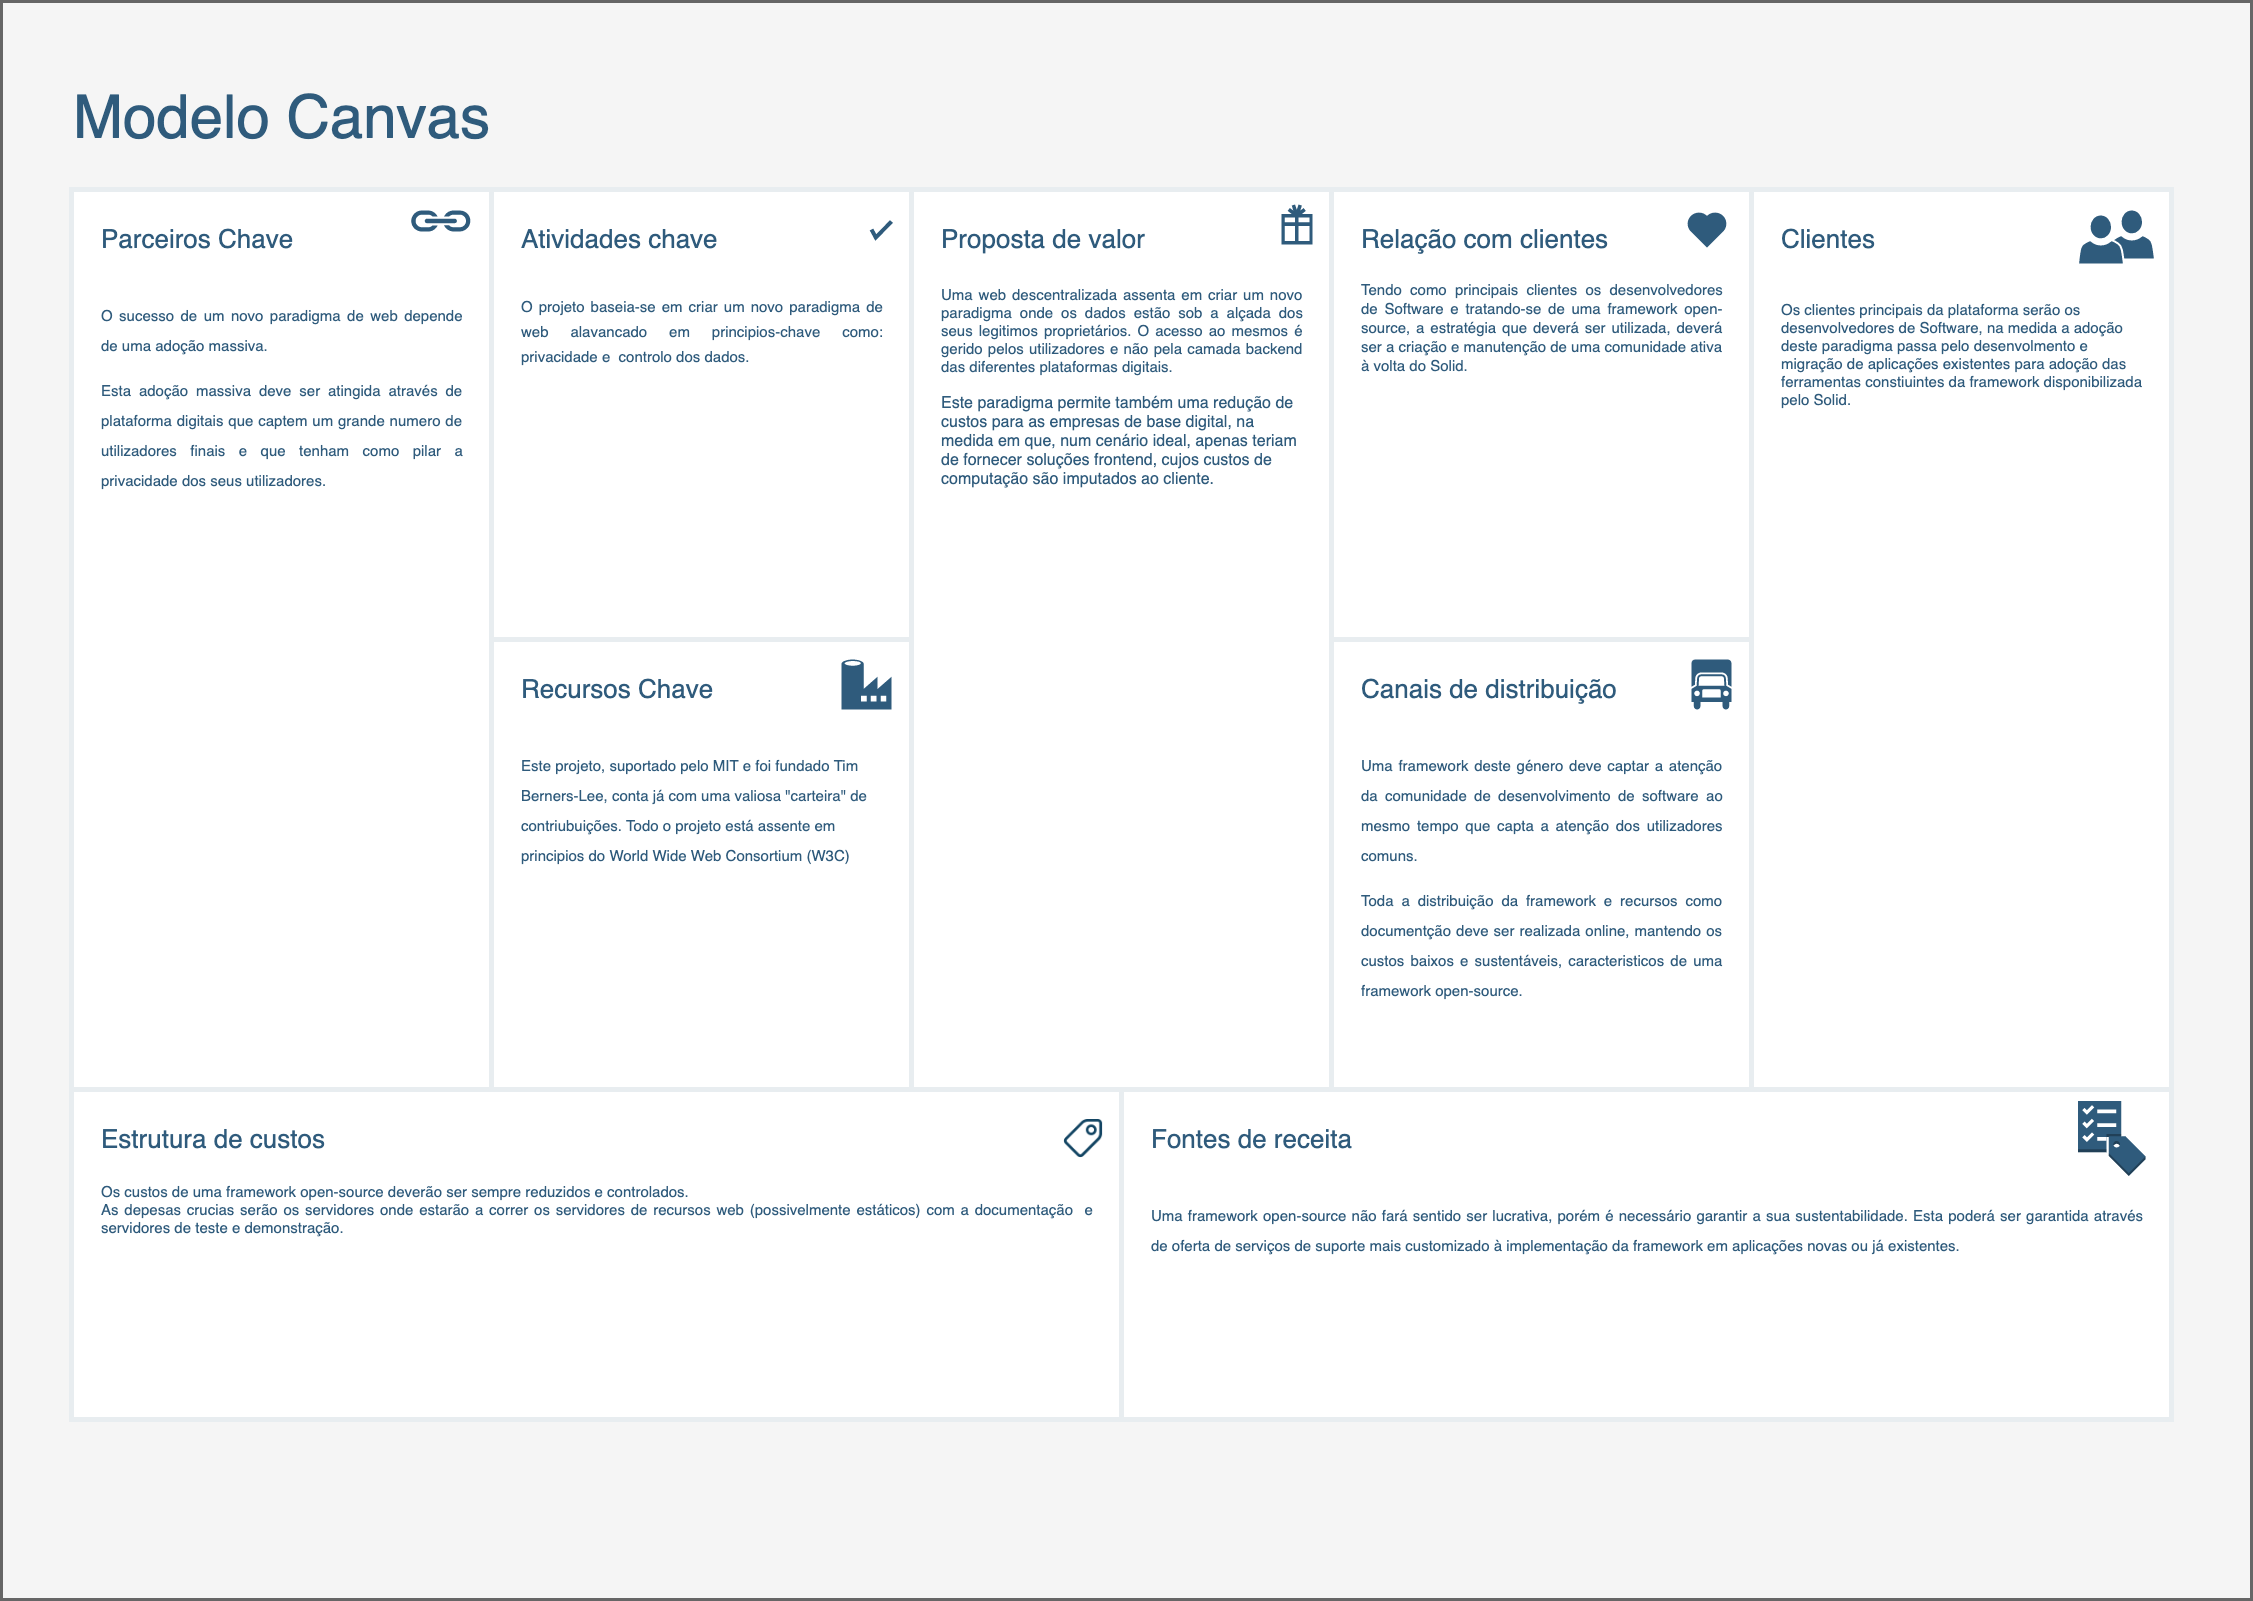
\includegraphics[height=0.9 \textwidth, angle=90]{figures/Canvas-Canvas.png}
    \caption{Modelo Canvas}
    \end{center}
\end{figure}

\section{Sumário}
Tendo por base o modelo de análise \emph{New Concept Development} e o processo de apoio à decisão \emph{AHP}, são apresentados dados que permitem concluir que o \emph{Solid} é o modelo descentralizado com maior potencial tendo em conta os parâmetros estabelecidos (\emph{c.f.} secção \ref{section_analise}).

A proposta de valor apresentada na secção \ref{section_proposta_de_valor} permite criar uma ideia geral da arquitetura e casos de uso que deverão ser desenhados no capítulo \ref{cap:4} de forma a melhorar o potencial da plataforma \emph{Solid}.

